\section{Теорема о числе маршрутов длины k из одной вершины в другую. Формулировка, 
доказательство. Применить теорему к графу.}

Пусть у графа $G(V,E)$, $|V|=n$, $A$ -- матрица смежности.
Рассмотрим матрицы $A^2,\dots,A^n$, обозначим символом $a_{ij}^{(k)}$ --
элементы матрицы $A^k$.

\begin{theorem}
    Количество маршрутов из $v_i$ в $v_j$ длины $k$ равно числу $a_{ij}^{(k)}$.
\end{theorem}

\begin{proof}
    С помощью методы математической индукции:
    \begin{enumerate}[left=0.0em, labelsep=1em, topsep=0.0em, itemsep=0pt, parsep=0.5em]
        \item $k=1, A=A^1$ \\
        $a_{ij}^{(1)} = s$, где $s$ -- количество ребер, соединяющих вершины $v_i$, $v_j$.
        Поэтому количество маршрутов из $v_i$ в $v_j$ длины 1 равно $s$.

        \item Пусть утвеждение верно для $A^k$ и число маршрутов длины $k$
        равно из $v_i$ в $v_j$ равно $a_{ij}^{(k)}$. Докажем справедливость
        для числа маршрутов длины $k+1$.
        \begin{align*}
            A^{k+1} = A^k \cdot A = 
            \begin{pmatrix}
                a_{11}^{(k)} & \dots & a_{1n}^{(k)}\\
                \hdotsfor[2]{3}\\
                a_{n1}^{(k)} & \dots & a_{nn}^{(k)}
            \end{pmatrix}
            \begin{pmatrix}
                a_{11} & \dots & a_{1n}\\
                \hdotsfor[2]{3}\\
                a_{n1} & \dots & a_{nn}
            \end{pmatrix}
        \end{align*}
        \begin{align*}
            a_{ij}^{(k+1)} = \sum_{t=1}^{n} a_{it}^{(k)}a_{tj}=
            a_{i1}^{(k)}a_{1j} + a_{i2}^{(k)}a_{2j} + \dots + a_{in}^{(k)}a_{nj}
        \end{align*}
        $a_{i1}^{(k)}$ -- количество маршрутов длины $k$ из $v_i$ в $v_1$, $a_{1j}$
        -- количество маршрутов из $v_1$ в $v_j$ длины 1 $\Rightarrow a_{i1}^{(k)}a_{1j}$
        -- количество маршрутов длины $k+1$ из $v_i$ в $v_j$, где последнее ребро $(v_1,v_j)$.
        
        Поскольку последнее ребро может быть либо $(v_1, v_j)$, либо $(v_2, v_j)$,
        либо $(v_n, v_j)$, то по правилу суммы в комбинаторике, получаем
        справедливость утверждения для $k + 1$.

        \item По методу математической индукции заключаем, что теорема верна
        для любого $n \in \mathbb{N}$.
    \end{enumerate}
\end{proof}

\newpage
В любом графе с $n$ вершинами расстояние от любой вершины до любой
другой не более $n-1$. Простой цикл в таком графе имеет длину не больше $n$.
Поэтому справедливы утверждения.

В графе (орграфе) $G$ с $n$ вершинами существует незамкнутый
маршрут из вершины $v_i$ в вершину $v_j$ $(v_i \neq v_j)$ тогда и только тогда, когда
элемент $b_{ij}$ матрицы $A + A^2 + \dots + A^{n-1}$ не равен 0.

В графе (орграфе) $G$ с $n$ вершинами тогда и только тогда
существует цикл, проходящий через вершину $v_i$, когда элемент $b_{ij}$ матрицы
$A + A^2 + \dots + A^n$ не равен нулю.

Пример теоремы к графу:
\begin{figure}[h]
    \centering
    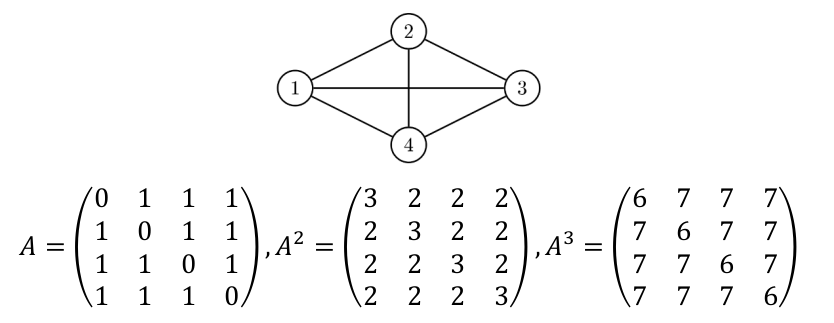
\includegraphics[scale=0.35]{17.png}
\end{figure}

Так как $a_{11}^{(2)}=3$, то существует ровно три маршрута из вершины
1 в 1 длиной 2.